%COMANDO CHE DETERMINA IL TIPO DI DOCUMENTO CHE SI VUOLE CREARE

\documentclass[a4paper,12pt]{report}

%ELENCO DEI PACCHETTI UTILI PER LA STESURA DEL DOCUMENTO

\usepackage[utf8]{inputenc}
\usepackage[english, italian]{babel}
\usepackage{graphicx}
\usepackage{float}
\usepackage{tabularx}
\usepackage{makecell}
\usepackage{titlesec}
\usepackage{fancyhdr}
\usepackage{lastpage}
\usepackage{xurl}
\usepackage{hyperref}
\usepackage{geometry}
\usepackage[table,dvipsnames]{xcolor}
\setcounter{tocdepth}{5}
\setcounter{secnumdepth}{5}
\usepackage{caption}
\usepackage{etoolbox}% >= v2.1 2011-01-03
\usepackage{tikz}
\usepackage{listings}
\usepackage{scalerel}
\usepackage{longtable}
\usepackage{comment}
\usepackage{amssymb}
\usepackage{listings}

\titleformat{\chapter}[display]
{\normalfont\bfseries}{}{0pt}{\LARGE}

%COMANDO PER LA SPAZIATURA DEI TITOLI DAL BORDO DEL FOGLIO

\titlespacing*{\chapter}{0cm}{0cm}{0.2cm}

%COMANDO PER LA SPAZIATURA DEL TESTO DAI BORDI LATERALI

\geometry{
	left=20mm,
	right=20mm,
}

%COMADNO PER AVERE L'INDICE DEL NOME CHE SI VUOLE

\renewcommand{\contentsname}{Indice}

%COMADNI PER OTTENERE SUBSUBSECTION NUMERATE E PRESENTI NELL'INDICE

\setcounter{tocdepth}{5}
\setcounter{secnumdepth}{5}

%COMANDI PER OTTENERE HEADER E FOOTER

\pagestyle{plain}

\fancypagestyle{plain}{
	\fancyhf{}
	\lhead{
\includegraphics[width=3cm]{../../immagini/minilogo.jpg}}
	\chead{}
	\rhead{\fontsize{12}{10}Verbale Esterno 2021-04-15}
	\lfoot{}
	\cfoot{\thepage\ di \pageref{LastPage}}
	\rfoot{}
}

\pagestyle{plain}

%COMANDI PER LINK

\hypersetup{
	colorlinks=true,
	linkcolor=black,
	filecolor=black,
	urlcolor=blue,
	citecolor=black,
}

%COMANDI PER SNIPPET DI CODICE

\BeforeBeginEnvironment{lstlisting}{\begin{mdframed}\vspace{-0.7em}}
	\AfterEndEnvironment{lstlisting}{\vspace{-0.5em}\end{mdframed}}

% needed for \lstcapt
\def\ifempty#1{\def\temparg{#1}\ifx\temparg\empty}

% make new caption command for listings
\usepackage{caption}
\newcommand{\lstcapt}[2][]{%
	\ifempty{#1}%
	\captionof{lstlisting}{#2}%
	\else%
	\captionof{lstlisting}[#1]{#2}%
	\fi%
	\vspace{0.75\baselineskip}%
}

\definecolor{atomlightorange}{rgb}{0.88,0.76,0.55}
\definecolor{atomdarkgrey}{RGB}{59,62,75}

% set listings
\lstset{%
	basicstyle=\footnotesize\ttfamily\color{atomlightorange},
	framesep=20pt,
	belowskip=10pt,
	aboveskip=10pt
}

% add frame environment
\usepackage[%
framemethod=tikz,
skipbelow=8pt,
skipabove=13pt
]{mdframed}
\mdfsetup{%
	leftmargin=0pt,
	rightmargin=0pt,
	backgroundcolor=atomdarkgrey,
	middlelinecolor=atomdarkgrey,
	roundcorner=6
}

%BIBLIOGRAFIA

\makeatletter
\def\thebibliography#1{\chapter*{Bibliografia\@mkboth
		{Bibliografia}{Bibliografia}}\list
	{[\arabic{enumi}]}{\settowidth\labelwidth{[#1]}\leftmargin\labelwidth
		\advance\leftmargin\labelsep
		\usecounter{enumi}}
	\def\newblock{\hskip .11em plus .33em minus .07em}
	\sloppy\clubpenalty4000\widowpenalty4000
	\sfcode`\.=1000\relax}
\makeatother

%DEFINIZIONE COLORI

\definecolor{airforceblue}{rgb}{0.36, 0.54, 0.66}


\begin{document}
	
	\makeatletter
	\begin{titlepage}
		\begin{center}
			\vspace*{-4cm}
			\author{Jawa Druids} 
			\title{Manuale Utente}
			\date{} %LASCIARE QUESTO CAMPO VUOTO, SE LO TOLGO STAMPA LA DATA CORRENTE
			
\includegraphics[width=0.5\linewidth]{../immagini/DRUIDSLOGO.jpg}\\[4ex]
			{\huge \bfseries  \@title }\\[2ex] 
			{\LARGE  \@author}\\[50ex]
			\vspace*{-9cm}
			\begin{table}[H]
				\renewcommand{\arraystretch}{1.4}
				\centering
				\begin{tabular}{r | l}
					\textbf{Versione} & 1.0.0 \\%RIGA PER INSERIRE LA VERSIONE ULTIMA DEL DOCUMENTO
					\textbf{Data approvazione} & \\
					\textbf{Responsabile} & Emma Roveroni\\
					\textbf{Redattori} & \makecell[tl]{ Emma Roveroni \\ Margherita Mitillo} \\
					\textbf{Verificatori} & \makecell[tl]{Igli Mezini \\ Andrea Cecchin \\ Emma Roveroni} \\
					%MAKECELL SERVE PER POI ANDARE A CAPO ALL'INTERNO DELLA CELLA
					\textbf{Stato} & \\
					\textbf{Lista distribuzione} & \makecell[tl]{Jawa Druids \\ Prof. Tullio Vardanega \\ Prof. Riccardo Cardin \\ Sync Lab}\\
					\textbf{Uso} & Esterno  
				\end{tabular}
			\end{table}
			\vspace{0.1cm}
			\hfill \break
			\fontsize{17}{10}\textbf{Sommario} \\
			\vspace{0.1cm}
			Il documento contiene il manuale destinato all'utente
		\end{center}
	\end{titlepage}
	\makeatother
	
	\quad
\begin{center}
	\LARGE\textbf{Registro delle modifiche}
\end{center}

\def\tabularxcolumn#1{m{#1}}
{\rowcolors{2}{RawSienna!90!RawSienna!20}{RawSienna!70!RawSienna!40}


\begin{center}
	\renewcommand{\arraystretch}{1.4}
	\begin{longtable}[c]{|p{2cm-1\tabcolsep}|p{2cm}|p{3cm-2\tabcolsep}|p{2,5cm-2\tabcolsep}|p{2,5cm}|p{4cm-2\tabcolsep}|}
		\hline
		\rowcolor{airforceblue}
		\makecell[c]{\textbf{Versione}} & \makecell[c]{\textbf{Data}} & \makecell[c]{\textbf{Autore}} & \makecell[c]{\textbf{Ruolo}} & \makecell[c]{\textbf{Verificatore}} & \makecell[c]{\textbf{Modifica}}\\
		\hline
		\centering v1.0.0 & 07-02-2021 & Andrea Dorigo & \centering \textit{Analista} & \centering - & \textit{Approvazione del documento} \\
		\hline
		\centering v0.1.0 & 05-02-2021 & Emma Roveroni & \centering \textit{Analista} & Andrea Cecchin & \textit{Revisione complessiva del documento} \\
		\hline
		\centering v0.0.1 & 03-02-2021 & Emma Roveroni & \centering \textit{Analista} & Andrea Cecchin & \textit{Stesura del documento} \\
		\hline
		
	\end{longtable}
\end{center}
	\tableofcontents{}
	\listoffigures
	\listoftables	
	
	\chapter{Introduzione}\label{Introduzione}

\section{Scopo del documento}
Il Piano di Qualifica è un documento su cui si prevede di operare per l’intera durata del progetto 
e il cui scopo è presentare e descrivere le strategie di verifica e validazione adottate 
dal gruppo Jawa Druids al fine di garantire la qualità di prodotto e di processo.  
Per raggiungere questo obbiettivo viene applicato un sistema di verifica continua sui processi in corso e 
sulle attività svolte, in modo da rilevare e correggere subito eventuali anomalie, riducendo lo spreco di risorse 
ed il rischio di reiterare gli stessi errori.
\section{Scopo del prodotto}
L'obiettivo del prodotto \textit{GDP - Gathering Detection Platform} di \textit{Sync Lab} è la creazione di un sistema software in 
grado di acquisire, monitorare, utilizzare e correlare tra loro tutti i dati acquisiti tramite sensoristica (come telecamere di videosorveglianza)
e altre sorgenti dati (es. orari con il maggior numero di visite degli esercizi commerciali estrapolati da Google) con lo
scopo di avere indicazioni di potenziali assembramenti e quindi di fornire supporto per trovare soluzioni che limitino tali condizioni.
\section{Glossario}
Al fine di favorire la comprensione totale della documentazione relativa al progetto, viene fornito un documento denominato \textit{Glossario -- fornire versione}
che riporta la spiegazione della terminologia specifica e tecnica utilizzata per la stesura di questo ed altri documenti.
Tali termini, quando utilizzati, vengono contrassegnati con un apice \textsuperscript{G} alla fine della parola.
\section{Standard di progetto}
Decidere se scrivere di aver utilizzato un determinato standard ISO per il software, se si, definirlo nelle norme di progetto!
\section{Riferimenti}
\subsection{Riferimenti normativi}
\begin{itemize}
	\item \textit{Norme di Progetto}
\end{itemize}
\subsection{Riferimenti informativi}
\begin{itemize}
	\item \textit{IEEE Recommended Practice for Software Requirements Specifications:}\\
	\url{https://ieeexplore.ieee.org/document/720574}
	\item \textit{Seminario per approfondimenti tecnici del capitolato C3:}\\
	\url{https://www.math.unipd.it/~tullio/IS-1/2020/Progetto/ST1.pdf}		
\end{itemize}
	\chapter{Requisiti di sistema ed installazione}\label{RequisitiDiSistemaEdInstallazione}

\section{Requisiti di sistema}\label{RequisitiDiSistemaEdInstallazioneRequisiti}
\textit{GDP - Gathering Detection Platform} è un'applicazione web$_{\scaleto{G}{3pt}}$ per dispositivi desktop ed è quindi utilizzabile con qualsiasi sistema operativo che supporti l'installazione dei broswer supportati(vedi \S~\ref{RequisitiDiSistemaEdInstallazioneRequisitiBrowserSupportati}). Tuttavia, per poter installare i moduli interni del nostro software$_{\scaleto{G}{3pt}}$, è consigliabile rispettare i seguenti requisiti hardware e software$_{\scaleto{G}{3pt}}$:

\subsection{Requisiti hardware}\label{RequisitiDiSistemaEdInstallazioneRequisitiRequisitiHardware}

Il software$_{\scaleto{G}{3pt}}$ è stato testato, con esito positivo, su una macchina con le seguenti caratteristiche:
\begin{itemize}
	\item RAM: 4Gb;
	\item hard disk: 10Gb;
	\item processore: Intel(R) Core(TM) i7-4710HQ CPU @ 2.50GHz CPU.
\end{itemize}
e su di un MacBook Air (early 2015) con le seguenti caratteristiche:
\begin{itemize}
	\item RAM: 4Gb;
	\item Solid State Drive: 128Gb;
	\item processore: Intel(R) Core(TM) i5 Dual Core @ 1.6GHz CPU.
	\item Mac OS v11.2.3
\end{itemize}

Nonostante non sia stato possibile fornire i requisiti minimi esatti a causa di mancanza di macchine fisiche, possiamo garantire che il software funzioni correttamente su macchine di specifiche simili o migliori.

\subsection{Browser supportati}\label{RequisitiDiSistemaEdInstallazioneRequisitiBrowserSupportati}
Perché l'applicazione funzioni in modo corretto, è necessario che Javascript$_G$ sia abilitato sul browser. 
Qui di seguito sono riportati i browser per i quali si garantisce la compatibilità. 
\begin{itemize}
	\item \textit{Google Chrome} versione 88 o superiore;
	\item \textit{Microsoft Edge} versione 87;
	\item \textit{Mozzilla Firefox Developer} versione 89;
	\item \textit{Safari} versione 14.0.3 o superiore.
\end{itemize}
L'applicazione web$_G$ potrebbe funzionare correttamente anche su versioni precedenti e/o successive o su altri browser, ma non si garantisce il supporto. 

\section{Procedure di installazione}\label{RequisitiDiSistemaEdInstallazioneInstallazione}
Questa sezione esporrà le procedure di installazione all'interno del sistema operativo Linux$_G$, più precisamente Ubuntu$_G$ 20.04 LTS, in quanto utilizzato anche per lo sviluppo del software$_{\scaleto{G}{3pt}}$ stesso.
Rimane comunque possibile installare il software$_{\scaleto{G}{3pt}}$ su altri sistemi operativi soddisfacendo le dipendenze necessarie, ma non verrà qui esplicitato.

\subsection{Download della  repository}\label{RequisitiDiSistemaEdInstallazioneInstallazioneDownloadRepo}
Per scaricare correttamente i contenuti della repository$_G$ è necessario installare \texttt{git} e \texttt{git-lfs} (\textit{Git Large File Storage}).
Su Ubuntu$_{\scaleto{G}{3pt}}$ 20.04 LTS, questo è possibile eseguendo il comando:
\begin{lstlisting}
sudo apt install git git-lfs
\end{lstlisting}
assumendo che le principali repository$_{\scaleto{G}{3pt}}$ per i pacchetti di Ubuntu$_{\scaleto{G}{3pt}}$ siano attive (Universe, Multiverse).

Questo passaggio è richiesto poiché GitHub$_G$ (il sito che ospita la repository$_{\scaleto{G}{3pt}}$ del progetto) consente l'upload di file con dimensioni massime fino a 100MB.
L'utilizzo di \textit{Git Large File Storage} permette l'upload e il download di file che superano questo limite, ed in particolare permette l'upload e download dei pesi necessari all'algoritmo YOLOv3 per il rilevamento di oggetti (più precisamente per il rilevamento delle persone in un'immagine), il quale ha una dimensione maggiore di 200MB. Maggiori informazioni riguardo \textit{Git Large File Storage} sono reperibili all'indirizzo:
\begin{center}
 \url{https://git-lfs.github.com} .
\end{center}

È dunque possibile scaricare correttamente la repository$_{\scaleto{G}{3pt}}$ relativa al progetto \textit{Gathering-Detection-Platform} con il seguente comando:
\begin{lstlisting}
git clone https://github.com/Andrea-Dorigo/gathering-detection-platform.git
\end{lstlisting}
% \begin{center}
%   \item \url{https://github.com/Andrea-Dorigo/gathering-detection-platform}
% \end{center}

\subsection{Installazione dipendenze}\label{RequisitiDiSistemaEdInstallazioneInstallazioneInstallazioneDipendenze}
Dopo aver eseguito il passo sopra descritto, bisogna installare le dipendenze necessarie a far eseguire il prodotto software$_{\scaleto{G}{3pt}}$ adeguatamente.
Per fare ciò è sufficiente aprire il terminale all'interno della cartella \textit{gathering-detection-platform}, ed eseguire i seguenti comandi:
\begin{lstlisting}
sudo apt install python3-opencv python3-pip mongodb maven npm
\end{lstlisting}
\begin{lstlisting}
pip3 install mongoengine
\end{lstlisting}
Per installare la dipendenza concernente a Kafka$_G$ si sono seguiti i passaggi presenti al seguente link:
\begin{center}
	\url{https://kafka.apache.org/quickstart}
\end{center}
Durante il suo processo di configurazione il nome del topic$_G$ da inserire è \textbf{gdp}.
Una volta concluse queste operazioni con esito positivo, il programma potrà essere eseguito.

\subsection{Inizializzazione modulo Acquisition}\label{RequisitiDiSistemaEdInstallazioneInstallazioneInizializzazioneModuloAcquisition}
Per eseguire il modulo di acquisizione, in modo da iniziare a raccogliere i dati dalle webcam salvate, basterà posizionarsi all'interno della cartella \texttt{acquisition/main/}, e da terminale eseguire il comando:
\begin{lstlisting}
python3 detect.py
python3 kafkaConsumer.py
\end{lstlisting}
Se i passi precedenti sono stati eseguiti correttamente, allora si visualizzeranno sul terminale i vari passaggi che svolge il modulo.


\subsection{Inizializzazione modulo Prediction}\label{RequisitiDiSistemaEdInstallazioneInstallazioneInizializzazioneModuloPrediction}
Per eseguire il modulo di predizione, che tramite il machine-learning$_G$ si occupa di calcolare le predizioni del periodo di tempo futuro, bisogna posizionarsi all'interno della cartella \texttt{prediction/} ed eseguire il seguente comando da terminale:

\begin{lstlisting}
python3 DataPrediction.py
\end{lstlisting}
In tal modo verrà attivato il modulo per le predizioni sui dati.
Saranno visibili sul terminale gli step eseguiti dal programma.

\subsection{Inizializzazione modulo Web-App}\label{RequisitiDiSistemaEdInstallazioneInstallazioneInizializzazioneModuloWebApp}
Per avviare la web-app$_G$, e le sue funzioni, si devono eseguire alcuni comandi, sempre da terminale, a partire dalla cartella \textit{webapp}.
\begin{enumerate}
	\item posizionarsi all'interno della cartella \texttt{webapp/} ed eseguire:
\begin{lstlisting}
mvn spring-boot:run
\end{lstlisting}
\item posizionarsi all'interno della cartella "vue-js-client-crud" ed eseguire:
\begin{lstlisting}
npm install
\end{lstlisting}
\item all'interno della stessa cartella bisogna eseguire:
\begin{lstlisting}
npm run serve
\end{lstlisting}
\item infine, la piattaforma \textit{Gathering-Detection-Platform} sarà disponibile all'indirizzo di default \url{http://localhost:8081} 
\end{enumerate}
Il primo comando inizializza il server di Spring$_G$ che fornisce i servizi per prelevare le informazioni dal database, mentre i comandi successivi installano i moduli necessari tramite npm$_G$ ed eseguono l'applicazione.


	<<<<<<< HEAD:documentazione/manuale_utente/capitolo/c3_Utilizzo_di_GDP.tex
\chapter{Utilizzo di GDP - Gathering Detection Platform}\label{UtilizzoDiGDPGatheringDetecionPlatform}

\section{Pagina iniziale}\label{UtilizzoDiGDPGatheringDetecionPlatformPaginaIniziale}
La pagina iniziale che si presenta all'avvio è mostrata nella seguente figura.
Al suo interno sono presenti le componenti di seguito elencate e spiegate ognuna in una sezione a se stante.
\begin{itemize}
	\item Il nome della web application;
	\item La barra di navigazione;
	\item Contenuto centrale;
	\item Il footer.
\end{itemize}

\section{Barra di navigazione}\label{UtilizzoDiGDPGatheringDetecionPlatformBarraDiNavigazione}

La barra di navigazione è quella rappresentata in figura n (mettere figura) ed è presente in tutte le pagine dell'applicazione web. Tramite questa l'utente potrà navigare all'interno della piattaforma. Nella barra di navigazione sono presenti:
\begin{enumerate}
	\item \textit{Home}: link alla pagina iniziale;
	\item \textit{Chi siamo}: link alla pagina "Chi siamo";
	\item \textit{Barra di ricerca}: attraverso la barra di ricerca è possibile cercare, e quindi selezionare tra quelle disponibili, la città di cui si è interessati a visualizzare i dati sulla heat-map$_G$. 
\end{enumerate}

\begin{center}
	\begin{figure}
		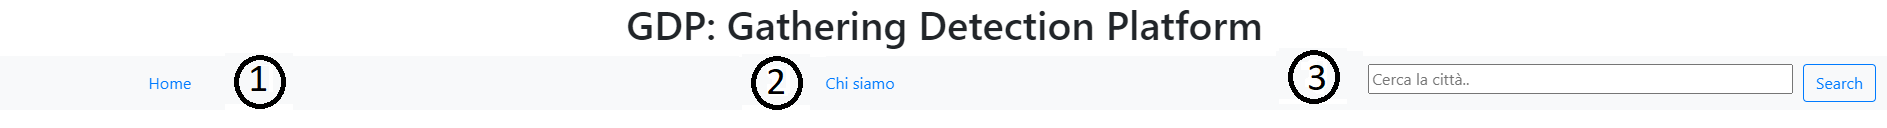
\includegraphics[width=1\linewidth]{../immagini/manualeUtente/BarraDiNavigazioe.png}
		\caption{Barra di Navigazione}
	\end{figure}
\end{center}

\section{Contenuto centrale}\label{UtilizzoDiGDPGatheringDetecionPlatformContenutoCentrale}
\subsection{Pagina Iniziale - Home} \label{UtilizzoDiGDPGatheringDetecionPlatformContenutoCentralePaginaInizialeHome}
La pagina iniziale che visualizza l'utente è quella mostrata in figura n (quella che c'è sopra in 3.1). 
\subsubsection{Heatmap}\label{UtilizzoDiGDPGatheringDetecionPlatformContenutoCentralePaginaInizialeHomeHeatmap}
Al centro della web app è presente una heat map$_{\scaleto{G}{3pt}}$ che raffigura, inizialmente, il flusso di persone presenti nella città di Roma nell'orario attuale. Successivamente l'utente potrà modificare la città, attraverso l'elenco delle città (\S~\ref{UtilizzoDiGDPGatheringDetecionPlatformContenutoCentralePaginaInizialeHomeMenùATendina}) oppure tramite la barra di ricerca, l'orario e la data, secondo quanto spiegato in \S~\ref{UtilizzoDiGDPGatheringDetecionPlatformContenutoCentralePaginaInizialeHomeCalendarioESlider}, e visualizzare tramite la heat map$_{\scaleto{G}{3pt}}$ i dati relativi ai campi selezionati.\\
Per facilitare la lettura della mappa, dopo che l'utente ha effettuato lo zoom-in, viene mostrato un pop-up, accompagnato da un marker, che evidenzia sia il nome del luogo che si sta osservando sia il numero di persone effettivamente presenti in quel momento. Questa funzionalità viene illustrata nella seguente figura n. (inserire figura pop-up)
\subsubsection{Elenco delle città} \label{UtilizzoDiGDPGatheringDetecionPlatformContenutoCentralePaginaInizialeHomeMenùATendina}

L'elenco delle città, posizionato a destra della mappa, viene utilizzato per la selezione della città. Infatti, l'utente, quando apre l'applicazione web, visualizza la mappa centrata sulla città di Roma, la città di default, ma successivamente può scegliere di osservare il flusso di persone relativo ad un'altra città presente tra quelle messe a disposizione nella lista. 
\begin{center}
	\begin{figure}
		\includegraphics[width=0.2\linewidth]{../immagini/manualeUtente/ElencoCittà.png}
		\caption{Elenco Città}
	\end{figure}
\end{center}

\subsubsection{Calendario e slider}\label{UtilizzoDiGDPGatheringDetecionPlatformContenutoCentralePaginaInizialeHomeCalendarioESlider}
L'utente ha a disposizione, a sinistra della mappa, un calendario che gli permette di scegliere l'anno, il mese ed il giorno di cui desidera visualizzare i dati. Per selezionare il mese bisogna spostarsi usando le freccie poste ai lati (1), mentre per l'anno si seleziona sull'anno corrente (2). \\
\begin{center}
	\begin{figure}
		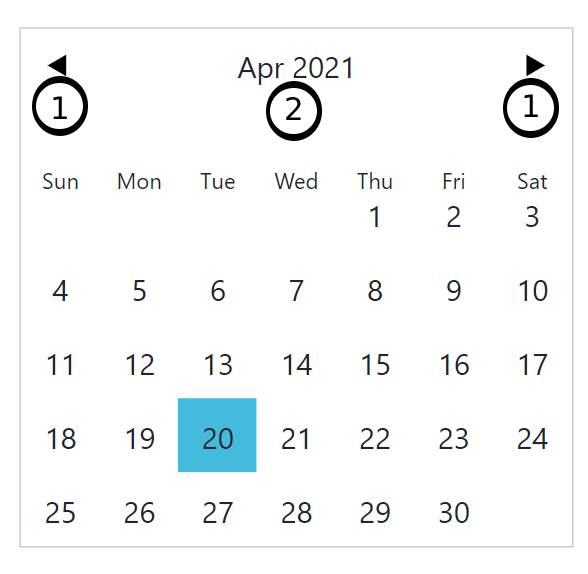
\includegraphics[width=0.3\linewidth]{../immagini/manualeUtente/Calendario.jpg}
		\caption{Calendario}
	\end{figure}
\end{center}
Al di sopra della mappa, invece, è presente uno slider con il quale l'utente può scegliere un orario diverso da quello attuale di cui desidera visualizzare i dati attraverso la heat map$_{\scaleto{G}{3pt}}$. La selezione dell'orario è effettuata su intervalli di tempo di ora in ora. Per selezionare l'ora attravero lo slider, si può sia cliccare sulla scritta dell'orario che si vuole selezionare sia spostare il tooltip (non so come si chiami) (1).
\begin{center}
	\begin{figure}
		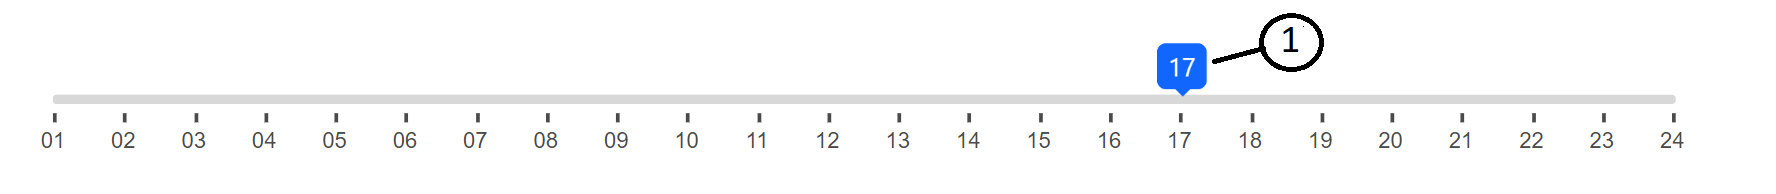
\includegraphics[width=1\linewidth]{../immagini/manualeUtente/Slider.png}
		\caption{Slider}
	\end{figure}
\end{center}

\subsubsection{Bottone Reload Map} \label{UtilizzoDiGDPGatheringDetecionPlatformContenutoCentralePaginaInizialeHomeBottoneReloadMap}
Nel caso in cui l'utente avesse selezionato una data diversa da quella odierna e/o un'ora differente da quella attuale, cliccando sul pulsante "Reload Map", la mappa si aggiornerà e tornerà a mostrare i dati in tempo reale, quindi relativi a data e ora corrente, rimanendo sulla città che si stava osservando. 
\begin{center}
	\begin{figure}
		
\includegraphics[width=0.3\linewidth]{../immagini/manualeUtente/ReloadMap.png}
		\caption{Reload Map}
	\end{figure}
\end{center}
\subsubsection{Messaggio d'errore} \label{UtilizzoDiGDPGatheringDetecionPlatformContenutoCentralePaginaInizialeHomeMessaggioDiErrore}
(inserire foto)
Nel caso in cui non ci siano dati disponibili nel database per il luogo, il giorno e l'ora in questione, l'utente visualizzerà un messaggio di errore che lo informerà del disguido e la mappa non mostrerà nessun dato. L'utente potrà chiudere il messaggio d'errore premendo il pulsante "OK". 
\begin{center}
	\begin{figure}
		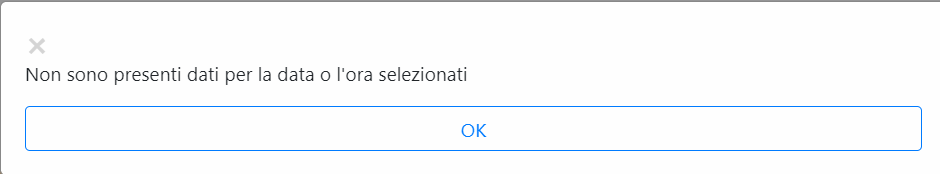
\includegraphics[width=0.5\linewidth]{../immagini/manualeUtente/MessaggioErrore.png}
		\caption{Messaggio d'errore}
	\end{figure}
\end{center}
\subsection{Chi siamo} \label{UtilizzoDiGDPGatheringDetecionPlatformContenutoCentraleChiSiamo}
(inserire immagine)\\
In questa pagina è possibile visualizzare le informazioni che riguardano il team di sviluppo JawaDruids, l'azienda proponente SyncLab e il progetto \textit{GDP: Gathering Detection Platform}. 
%da completare 

\section{Footer}\label{UtilizzoDiGDPGatheringDetecionPlatformFooter}
Il footer è presente in tutte le pagine dell'applicazione web e riporta alcuni link utili, come quello del sito web dell'azienda SyncLab e la mail del team di sviluppo, da contattare in caso si riscontrino problemi con l'uso del prodotto software. 
%da sistemare
\begin{center}
	\begin{figure}
		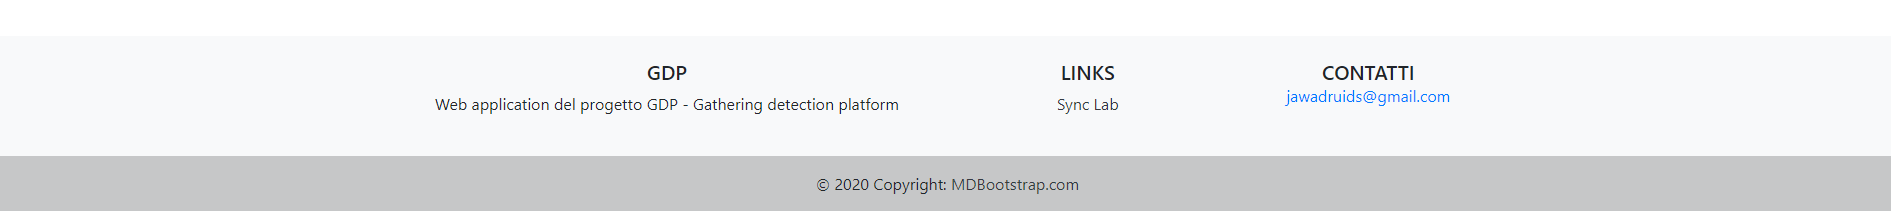
\includegraphics[width=1\linewidth]{../immagini/manualeUtente/Footer.png}
		\caption{Footer}
	\end{figure}
\end{center}


%COSE DA VALUTARE SE SCRIVERE O MENO
%1) che la mappa si aggiorna ogni 10 minuti automaticamente??? (ancora da implementare in realtà)
%2) parte di predizione?? slider +2 ore rispetto a quella attuale
=======
\chapter{Utilizzo di GDP - Gathering Detection Platform}\label{UtilizzoDiGDPGatheringDetecionPlatform}

\section{Pagina iniziale}\label{UtilizzoDiGDPGatheringDetecionPlatformPaginaIniziale}
La pagina iniziale che si presenta all'avvio è mostrata nella seguente figura.
Al suo interno sono presenti le componenti di seguito elencate e spiegate ognuna in una sezione a se stante.
\begin{itemize}
	\item Il nome della web application$_G$;
	\item La barra di navigazione;
	\item Contenuto centrale;
	\item Il footer$_g$.
\end{itemize}

\section{Barra di navigazione}\label{UtilizzoDiGDPGatheringDetecionPlatformBarraDiNavigazione}

La barra di navigazione è quella rappresentata in figura n (mettere figura) ed è presente in tutte le pagine dell'applicazione web$_{\scaleto{G}{3pt}}$. Tramite questa l'utente potrà navigare all'interno della piattaforma. Nella barra di navigazione sono presenti:
\begin{itemize}
	\item \textit{Home}: link alla pagina iniziale;
	\item \textit{Chi siamo}: link alla pagina "Chi siamo";
	\item \textit{Barra di ricerca}: attraverso la barra di ricerca è possibile cercare, e quindi selezionare tra quelle disponibili, la città di cui si è interessati a visualizzare i dati sulla heat-map$_G$. 
\end{itemize}
(inserire riferimenti tra elenco e ciò che si mostra nella foto?)
%scaricare il manuale utente ?????

\section{Contenuto centrale}\label{UtilizzoDiGDPGatheringDetecionPlatformContenutoCentrale}
\subsection{Pagina Iniziale - Home} \label{UtilizzoDiGDPGatheringDetecionPlatformContenutoCentralePaginaInizialeHome}
La pagina iniziale che visualizza l'utente è quella mostrata in figura n (quella che c'è sopra in 3.1). 
\subsubsection{Heatmap}\label{UtilizzoDiGDPGatheringDetecionPlatformContenutoCentralePaginaInizialeHomeHeatmap}
Al centro della web app$_{\scaleto{G}{3pt}}$ è presente una heat map$_{\scaleto{G}{3pt}}$ che raffigura, inizialmente, il flusso di persone presenti nella città di Roma nell'orario attuale. Successivamente l'utente potrà modificare la città, attraverso l'elenco delle città (\S~\ref{UtilizzoDiGDPGatheringDetecionPlatformContenutoCentralePaginaInizialeHomeMenùATendina}) oppure tramite la barra di ricerca, l'orario e la data, secondo quanto spiegato in \S~\ref{UtilizzoDiGDPGatheringDetecionPlatformContenutoCentralePaginaInizialeHomeCalendarioESlider}, e visualizzare tramite la heat map$_{\scaleto{G}{3pt}}$ i dati relativi ai campi selezionati.\\
Per facilitare la lettura della mappa, dopo che l'utente ha effettuato lo zoom-in$_G$, viene mostrato un pop-up$_G$, accompagnato da un marker$_G$, che evidenzia sia il nome del luogo che si sta osservando sia il numero di persone effettivamente presenti in quel momento. Questa funzionalità viene illustrata nella seguente figura n. (inserire figura pop-up)
\subsubsection{Elenco delle città} \label{UtilizzoDiGDPGatheringDetecionPlatformContenutoCentralePaginaInizialeHomeMenùATendina}
(inserire immagine) \\
L'elenco delle città, posizionato a destra della mappa, viene utilizzato per la selezione della città. Infatti, l'utente, quando apre l'applicazione web, visualizza la mappa centrata sulla città di Roma, la città di default, ma successivamente può scegliere di osservare il flusso di persone relativo ad un'altra città presente tra quelle messe a disposizione nella lista. 

\subsubsection{Calendario e slider}\label{UtilizzoDiGDPGatheringDetecionPlatformContenutoCentralePaginaInizialeHomeCalendarioESlider}
(inserire immagine caledario e slider) \\
L'utente ha a disposizione, a sinistra della mappa, un calendario che gli permette di scegliere l'anno, il mese ed il giorno di cui desidera visualizzare i dati. Per selezionare l'anno bisogna cliccare su 1 (da evidenziare nella figura i vari punti in cui cliccare per cambiare anno/mese/giorno) e per il mese 2.
%da scrivere che può solo andare nel passato e presente?
\\
Al di sopra della mappa, invece, è presente uno slider$_G$ con il quale l'utente può scegliere un orario diverso da quello attuale di cui desidera visualizzare i dati attraverso la heat map$_{\scaleto{G}{3pt}}$. La selezione dell'orario è effettuata su intervalli di tempo di ora in ora. 

\subsubsection{Bottone Reload Map} \label{UtilizzoDiGDPGatheringDetecionPlatformContenutoCentralePaginaInizialeHomeBottoneReloadMap}
(inserire immagine)\\
Nel caso in cui l'utente avesse selezionato una data diversa da quella odierna e/o un'ora differente da quella attuale, cliccando sul pulsante "Reload Map", la mappa si aggiornerà e tornerà a mostrare i dati in tempo reale, quindi relativi a data e ora corrente, rimanendo sulla città che si stava osservando. 
\subsubsection{Messaggio d'errore} \label{UtilizzoDiGDPGatheringDetecionPlatformContenutoCentralePaginaInizialeHomeMessaggioDiErrore}
(inserire foto)
Nel caso in cui non ci siano dati disponibili nel database per il luogo, il giorno e l'ora in questione, l'utente visualizzerà un messaggio di errore che lo informerà del disguido e la mappa non mostrerà nessun dato. L'utente potrà chiudere il messaggio d'errore tramite 1 e 2 (immagine)
\subsection{Chi siamo} \label{UtilizzoDiGDPGatheringDetecionPlatformContenutoCentraleChiSiamo}
(inserire immagine)\\
In questa pagina è possibile visualizzare le informazioni che riguardano il team di sviluppo \textit{Jawa Druids}, l'azienda proponente \textit{Sync Lab} e il progetto \textit{GDP: Gathering Detection Platform}. 
%da completare 

\section{Footer}\label{UtilizzoDiGDPGatheringDetecionPlatformFooter}
(inserire foto ??) \\
Il footer$_{\scaleto{G}{3pt}}$ è presente in tutte le pagine dell'applicazione web e riporta alcuni link utili, come quello del sito web dell'azienda \textit{Sync Lab} e la mail del team di sviluppo, da contattare in caso si riscontrino problemi con l'uso del prodotto software$_G$. 
%da sistemare


%COSE DA VALUTARE SE SCRIVERE O MENO
%1) che la mappa si aggiorna ogni 10 minuti automaticamente??? (ancora da implementare in realtà)
%2) parte di predizione?? slider +2 ore rispetto a quella attuale
>>>>>>> manuale_utente:documentazione/manuale_utente/capitoli/c3_Utilizzo_di_GDP.tex

	\chapter{Glossario} \label{Glossario}
\textbf{A} \\
\\
\textbf{Applicazione web} \\
Con applicazione web si intende un'applicazione accessibile via web attraverso un network. \\
\\
\textbf{F} \\
\\
\textbf{Footer} \\
Il footer indica la parte inferiore di un sito e normalmente ha lo stesso aspetto per tutte le pagine del dominio.Tipicamente contiene i link alle note legali, email  e ad altri elementi di navigazione del sito. \\
\\
\textbf{H} \\
\\
\textbf{Heat map} \\
 Rappresentazione grafica dei dati dove i singoli valori contenuti in una matrice sono rappresentati da colori. \\
\\
\textbf{J} \\
\\
\textbf{Java} \\
Linguaggio di programmazione ad alto livello, orientato agli oggetti e a tipizzazione statica, che si appoggia sull'omonima piattaforma software di esecuzione, specificatamente progettato per essere il più possibile indipendente dalla piattaforma hardware di esecuzione. Le principali caratteristiche di Java sono la portabilità, cioè il codice sorgente
è compilato in bytecode e può essere eseguito su ogni PC che ha JVM (Java Virtual Machine), e la robustezza. \\
\\
\\
\textbf{L} \\
\\
\textbf{Linux} \\
Linux è una famiglia di sistemi operativi open source che hanno come caratteristica comune quella di utilizzare come nucleo il kernel Linux. Linux è il primo rappresentante del software "libero", ovvero quel software che viene distribuito con una licenza che ne permette l'utilizzo da parte di chiunque. \\
\\
\textbf{N}\\
\\
\textbf{Node.js} \\
Node.js è un’applicazione, per la precisione un framework, che viene usata per scrivere applicazioni in Javascript lato server. \\
\\
\textbf{R} \\
\\
\textbf{Repository} \\
Ambiente di un sistema informativo in cui vengono conservati e gestiti file, documenti e metadati relativi ad un’attività di progetto. \\
\\
\textbf{S} \\
\\
\textbf{Slider} \\
Lo slider è un componente grafico usato dall'utente come cursore per regolare una proprietà. Infatti, attraverso tale componente, un utente può impostare un valore muovendo un indicatore, solitamente con uno spostamento orizzontale. In alcuni casi, l'utente può anche cliccare in un punto dello slider per cambiare le impostazioni.  \\
\\
\textbf{Software} \\
Un software èl'insieme delle procedure e delle istruzioni in un sistema di elaborazione dati. In contrapposizione all'hardware, si identifica con un insieme di programmi. \\
\\
\textbf{U} \\
\\
\textbf{Ubuntu} \\
\\
Ubuntu è un sistema operativo di distribuzione Linux, basata su Debian e che ha in Unity il suo ambiente desktop. Si basa esclusivamente su software libero distribuito liberamente con licenza GNU GPL ma supporta anche software proprietario. \\
\\
\textbf{V}\\
\\
\textbf{Vue.js}\\
 Framework open-source per lo sviluppo di applicazioni web, interfacce utente e applicazioni. \\
\\
\textbf{W} \\
\\
\textbf{Web application o web app}\\
\textit{Si rimanda alla voce "Applicazione web".}
	
\end{document}
